
\chapter{Introduction}

(UNDER MAJOR RESTRUCTURING, PLEASE WAIT FOR VERSION 2)

\url{http://www.libembroidery.org}

Embroidermodder is a free machine embroidery application.
The newest version, Embroidermodder 2 can:

\begin{itemize}
\item edit and create embroidery designs
\item estimate the amount of thread and machine time needed to stitch a design
\item convert embroidery files to a variety of formats
\item upscale or downscale designs
\item run on Windows, Mac and Linux
\end{itemize}

Embroidermodder 2 is very much a work in progress since we're doing a ground
up rewrite to an interface in C using the GUI toolkit SDL2.
The reasoning for this is detailed in the issues tab.

For a more in-depth look at what we are developing read
our [website]\url{https://www.libembroidery.org} which includes these docs as well as the up-to date printer-friendly versions.
These discuss recent changes, plans and has user and developer guides for all the Embroidermodder projects.

To see what we're focussing on right now, see the [Open Collective News]\url{https://opencollective.com/embroidermodder}.

The current printer-friendly version of the manual: \url{https://www.libembroidery.org/embroidermodder_2.0.0-alpha_manual.pdf}.

\section{License}

The source code is under the terms of the zlib license: see \texttt{LICENSE.md} in the source code directory.

Permission is granted to copy, distribute and/or modify this document
under the terms of the GNU Free Documentation License, Version 1.3
or any later version published by the Free Software Foundation;
with no Invariant Sections, no Front-Cover Texts, and no Back-Cover Texts.

A copy of the license is included in the section entitled ``GNU Free Documentation License''.


\section{The Embroidermodder Project and Team}

The \textit{Embroidermodder 2} project is a collection of small software utilities for
manipulating, converting and creating embroidery files in all major embroidery
machine formats. The program \textit{Embroidermodder 2} itself is a larger graphical
user interface (GUI) which is at the heart of the project.

The tools and associated documents are:

\begin{itemize}
\item This manual.
\item The website ([`www.libembroidery.org`](https://www.libembroidery.org)), which is maintained [here]\url{https://github.com/Embroidermodder/embroidermodder.github.io}.
\item Mobile embroidery format viewers and tools (`EmbroideryMobile`).
\item The core library of functions (`libembroidery`) and its manual.
\item The Python version of the library of functions (`libembroidery-python`) which is part of [libembroidery]\url{https://github.com/Embroidermodder/libembroidery}.
\item The CLI (`embroider`) which is part of [libembroidery]\url{https://github.com/Embroidermodder/libembroidery}.
\item Specs for an open hardware embroidery machine called Embroiderbot (not started yet) which is part of [libembroidery]\url{https://github.com/Embroidermodder/libembroidery} and its manual.
\item The GUI (`embroidermodder`), this repository.
\end{itemize}

They all tools to make the standard
user experience of working with an embroidery machine better without expensive
software which is locked to specific manufacturers and formats. But ultimately
we hope that the core \emph{Embroidermodder 2} is a practical, ever-present tool in
larger workshops, small cottage industry workshops and personal hobbyist's
bedrooms.

Embroidermodder 2 is licensed under the zlib license and we aim to keep all of
our tools open source and free of charge. If you would like to support the
project check out our [Open Collective](https://opencollective.com/embroidermodder) group. If you would like to help, please
join us on GitHub. This document is written as developer training as well
helping new users (see the last sections) so this is the place to learn how
to start changing the code.

The Embroidermodder Team is the collection of people who've submitted
patches, artwork and documentation to our three projects.
The team was established by Jonathan Greig and Josh Varga.
The full list is actively maintained below.

\section{Credits for Embroidermodder 2, libembroidery and all other related code}

If you have contributed and wish to be added to this list, alter the [README on Embroidermodder github page]\url{https://github.com/Embroidermodder/Embroidermodder} and we'll copy it to the libembroidery source code since that is credited to "The Embroidermodder Team".

\section{Embroidermodder 1}

The Embroidermodder Team is also inspired by the original Embroidermodder that was built by Mark Pontius and the same Josh Varga on SourceForge which unfortunately appears to have died from linkrot. We may create a distribution on here to be the official "legacy" Embroidermodder code but likely in a seperate repository because it's GNU GPL v3 and this code is written to be zlib (that is, permissive licensed) all the way down.

One reason why this is useful is that the rewrite by Jonathan Greig, John Varga and Robin Swift for Embroidermodder 2 should have no regressions: no features present in v1 should be missing in v2.

\section{Features}

Embroidermodder 2 has many advanced features that enable you to create awesome designs quicker, tweak existing designs to perfection, and can be fully customized to fit your workflow.

A summary of these features:

\begin{itemize}
\item Cross Platform
\item Realistic rendering
\item Various grid types and auto-adjusting rulers
\item Many measurement tools
\item Add text to any design
\item Supports many formats
\item Batch Conversion
\item Scripting API
\end{itemize}

\subsection{Cross Platform}

If you use multiple operating systems, it's important to choose software that works on all of them.

Embroidermodder 2 runs on Windows, Linux and Mac OS X. Let's not forget the Raspberry Pi (\url{http://www.raspberrypi.org}).

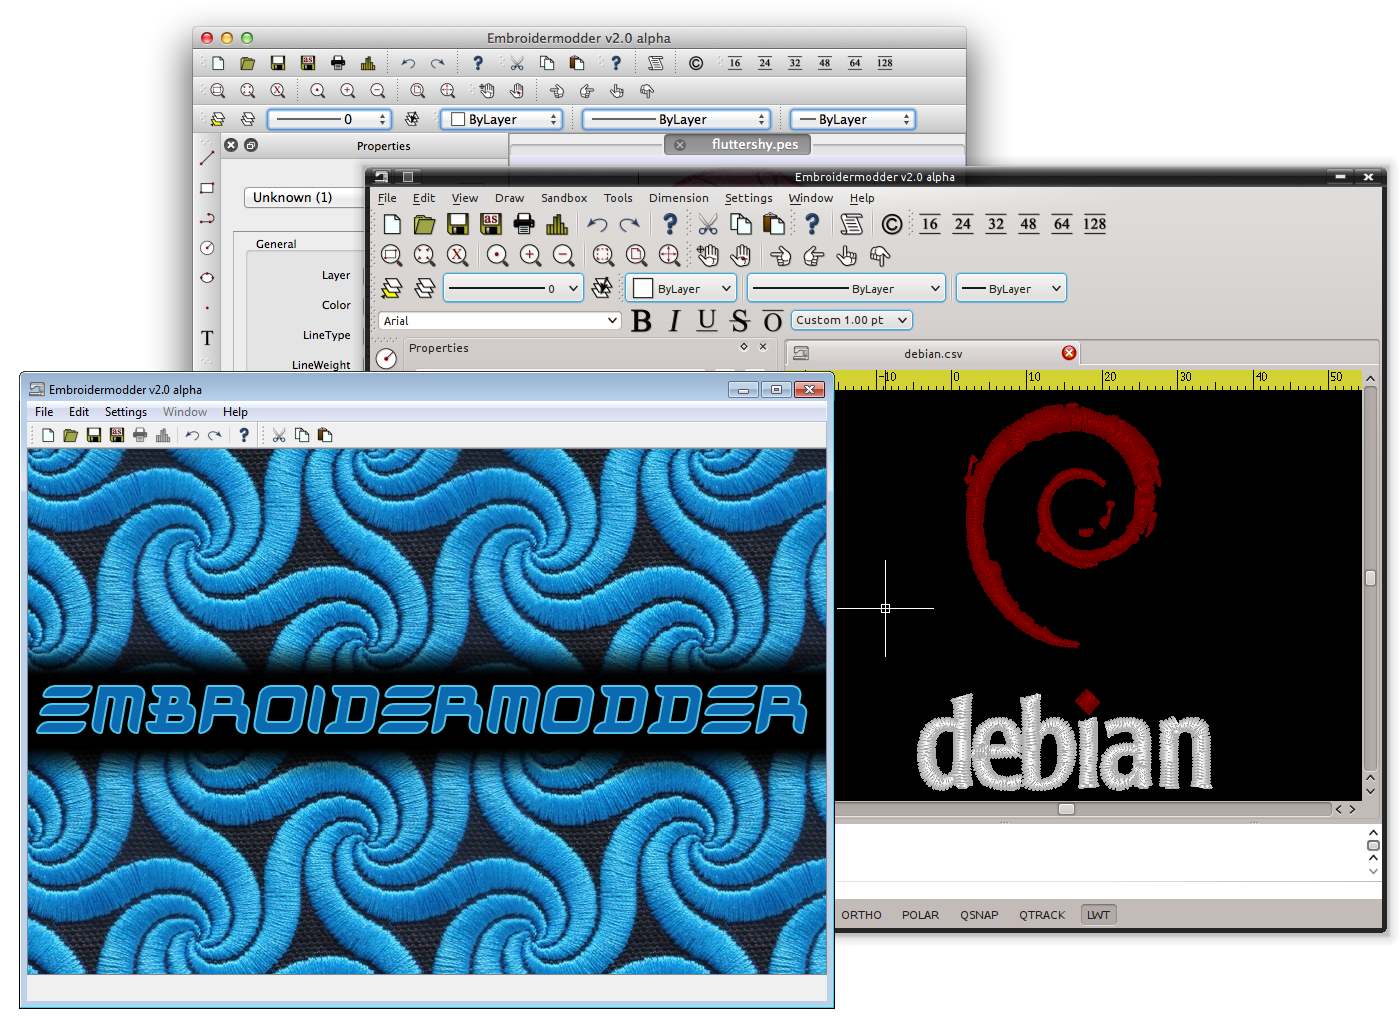
\includegraphics[width=0.9\textwidth]{images/features-platforms-1.png}

\section{Realistic Rendering}

It is important to be able to visualize what a design will look like when stitched and our pseudo ``3D'' realistic rendering helps achieve this.

Realistic rendering sample \#1:

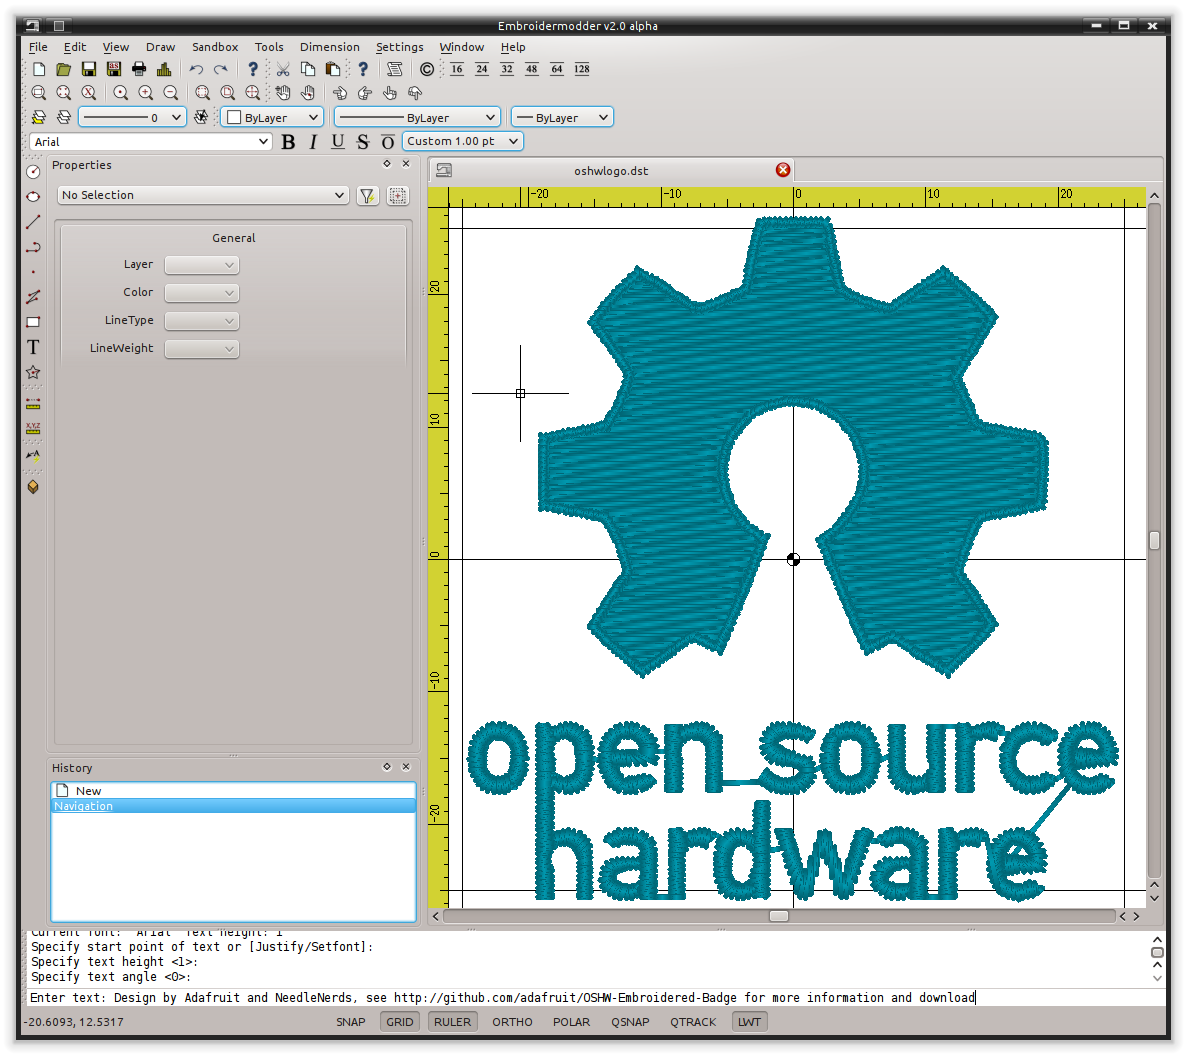
\includegraphics[width=0.9\textwidth]{images/features-realrender-1.png}

Realistic rendering sample \#2:

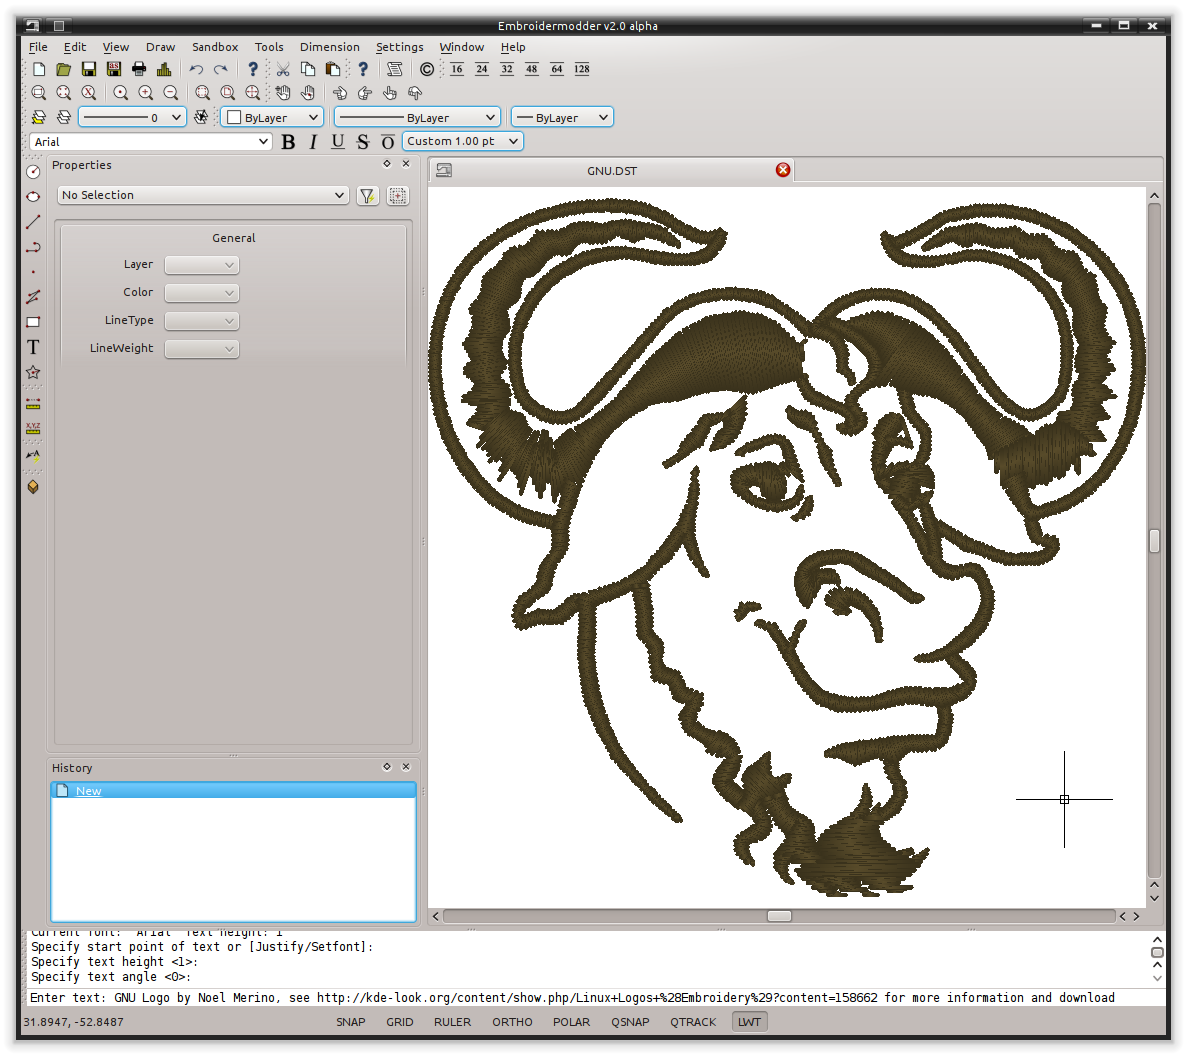
\includegraphics[width=0.9\textwidth]{images/features-realrender-2.png}

Realistic rendering sample \#3:

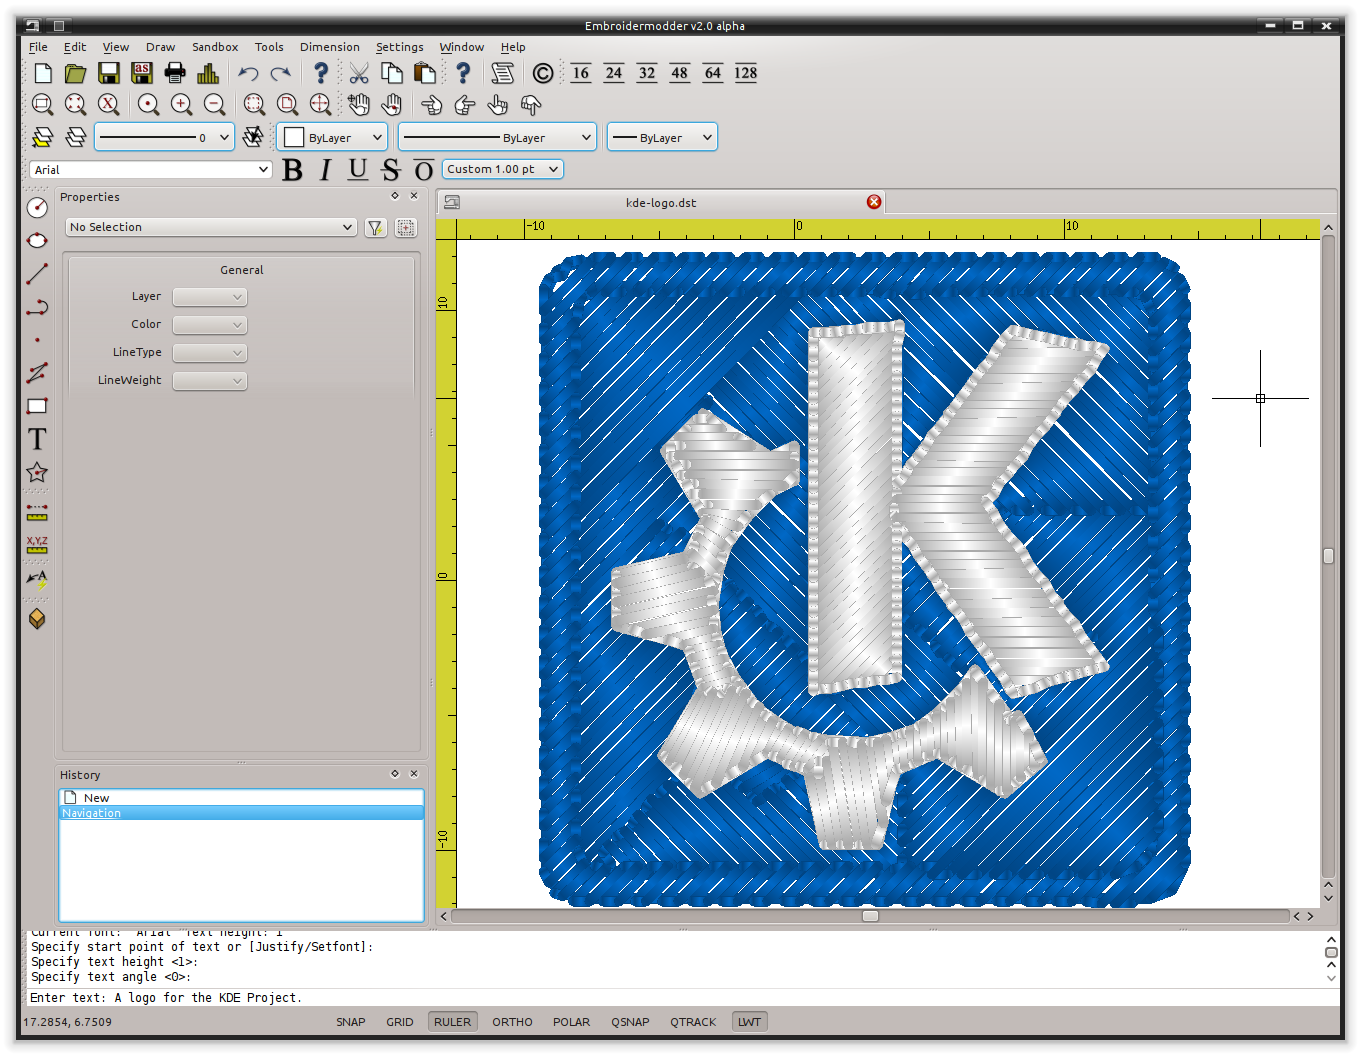
\includegraphics[width=0.9\textwidth]{images/features-realrender-3.png}

Various grid types and auto-adjusting rulers

Making use of the automatically adjusting ruler in conjunction with the grid will ensure your design is properly sized and fits within your embroidery hoop area.

Use rectangular, circular or isometric grids to construct your masterpiece!

Multiple grids and rulers in action:

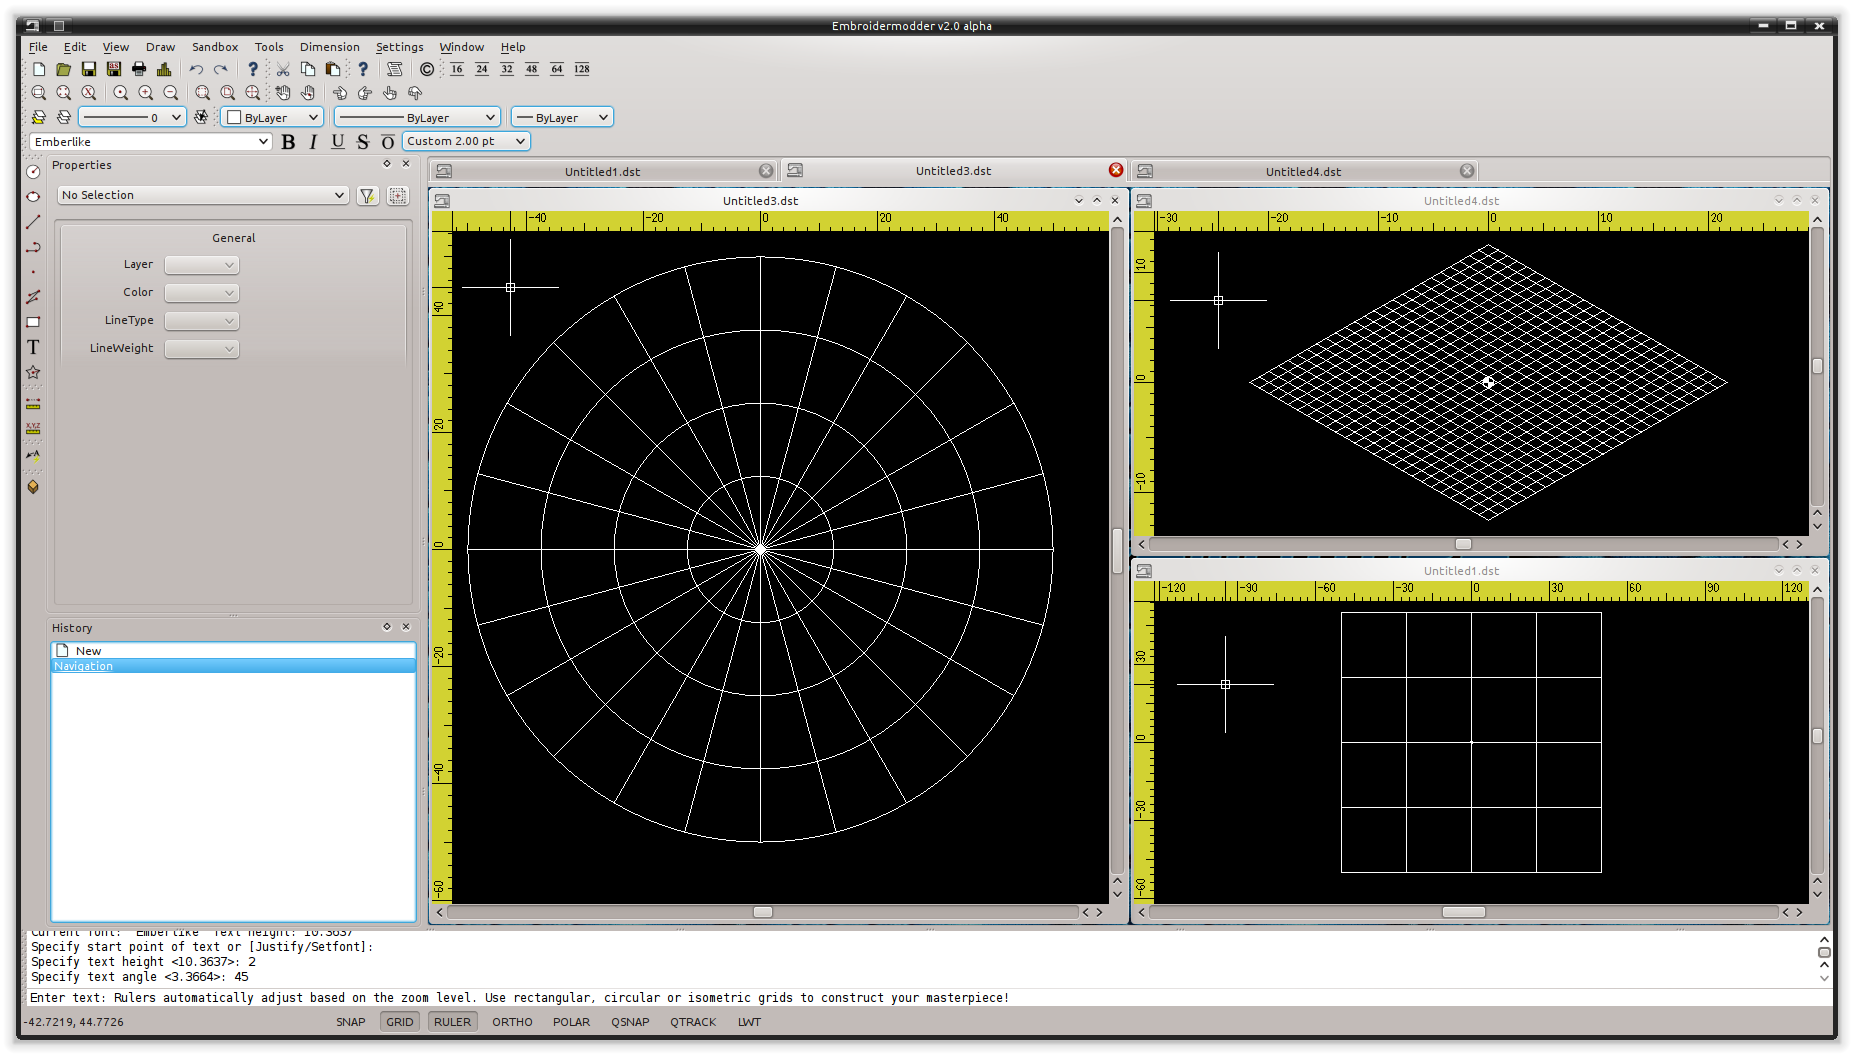
\includegraphics[width=0.9\textwidth]{images/features-grid-ruler-1.png}

\subsection{Many measurement tools}

Taking measurements is a critical part of creating great designs. Whether you are designing mission critical embroidered space suits for NASA or some other far out design for your next meet-up, you will have precise measurement tools at your command to make it happen. You can locate individual points or find distances between any 2 points anywhere in the design!

Take quick and accurate measurements:

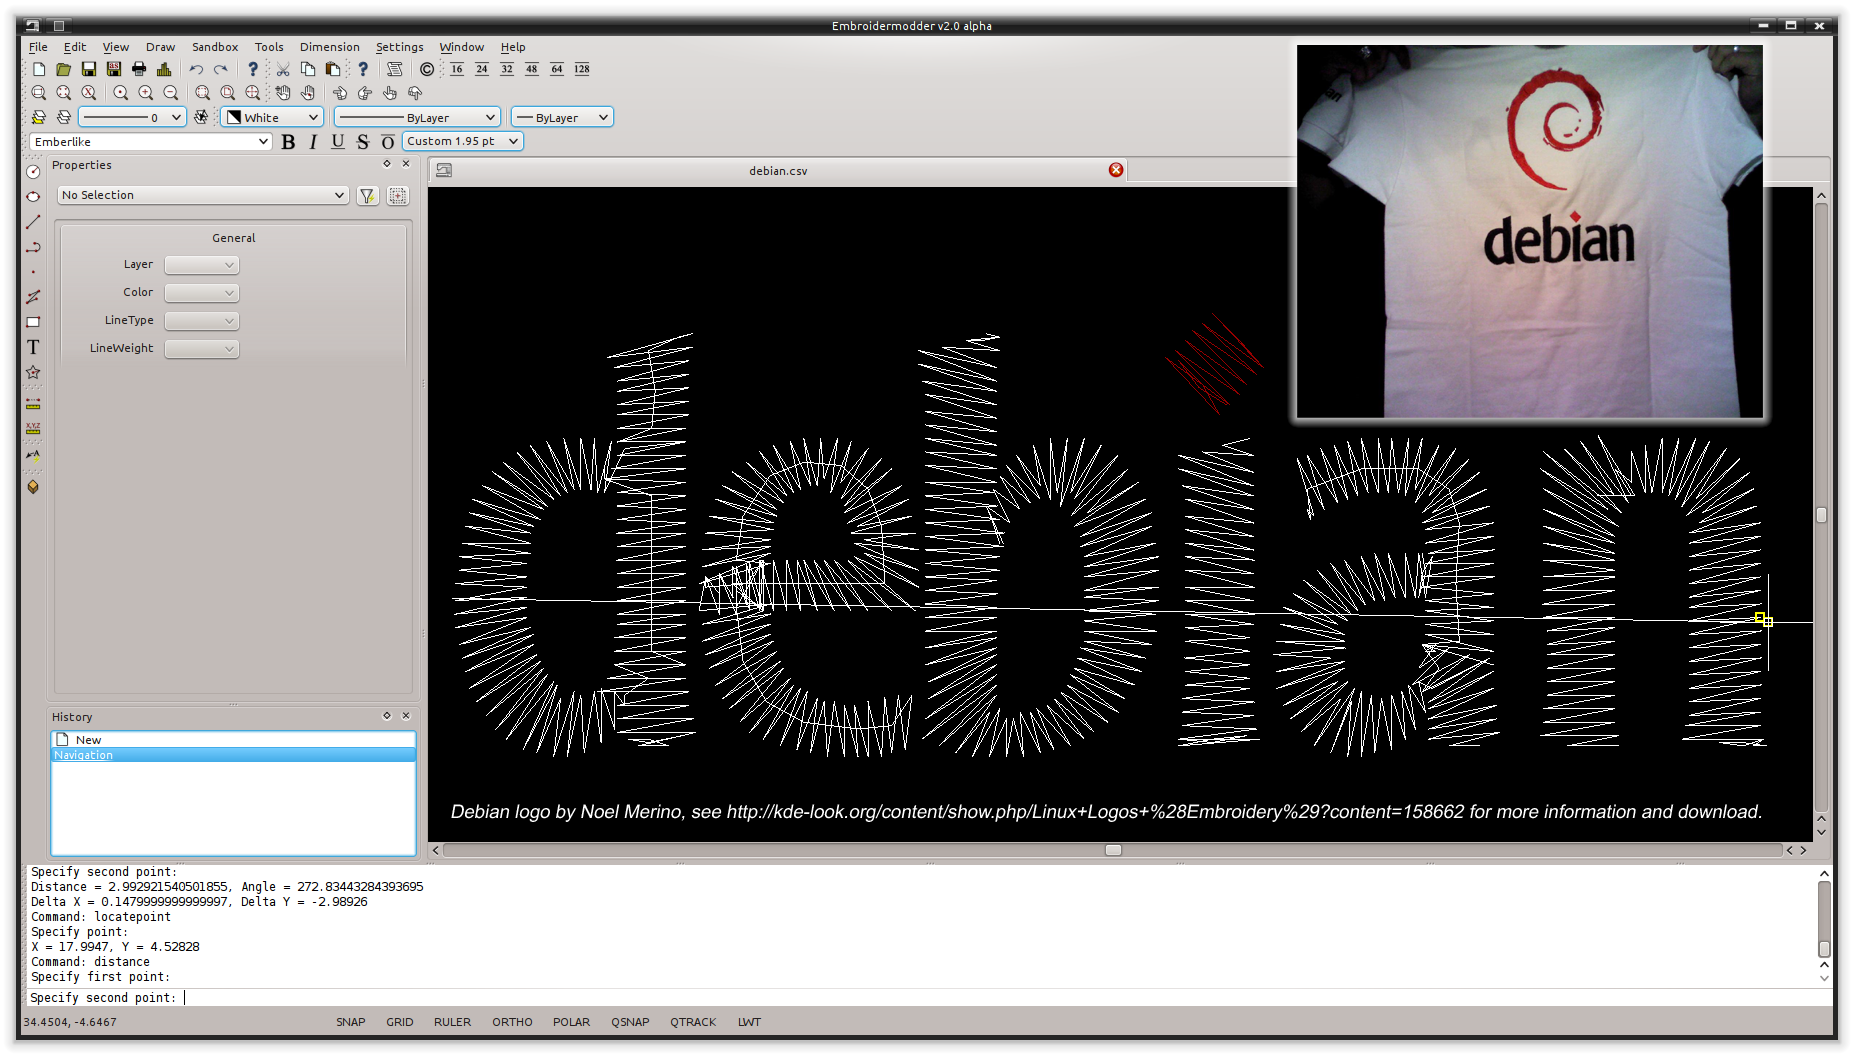
\includegraphics[width=0.9\textwidth]{images/features-measure-1.png}

\subsection{Add text to any design}

Need to make company apparel for all of your employees with individual names on them? No sweat. Just simply add text to your existing design or create one from scratch, quickly and easily.
Didn't get it the right size or made a typo? No problem. Just select the text and update it with the property editor.

Add text and adjust its properties quickly:

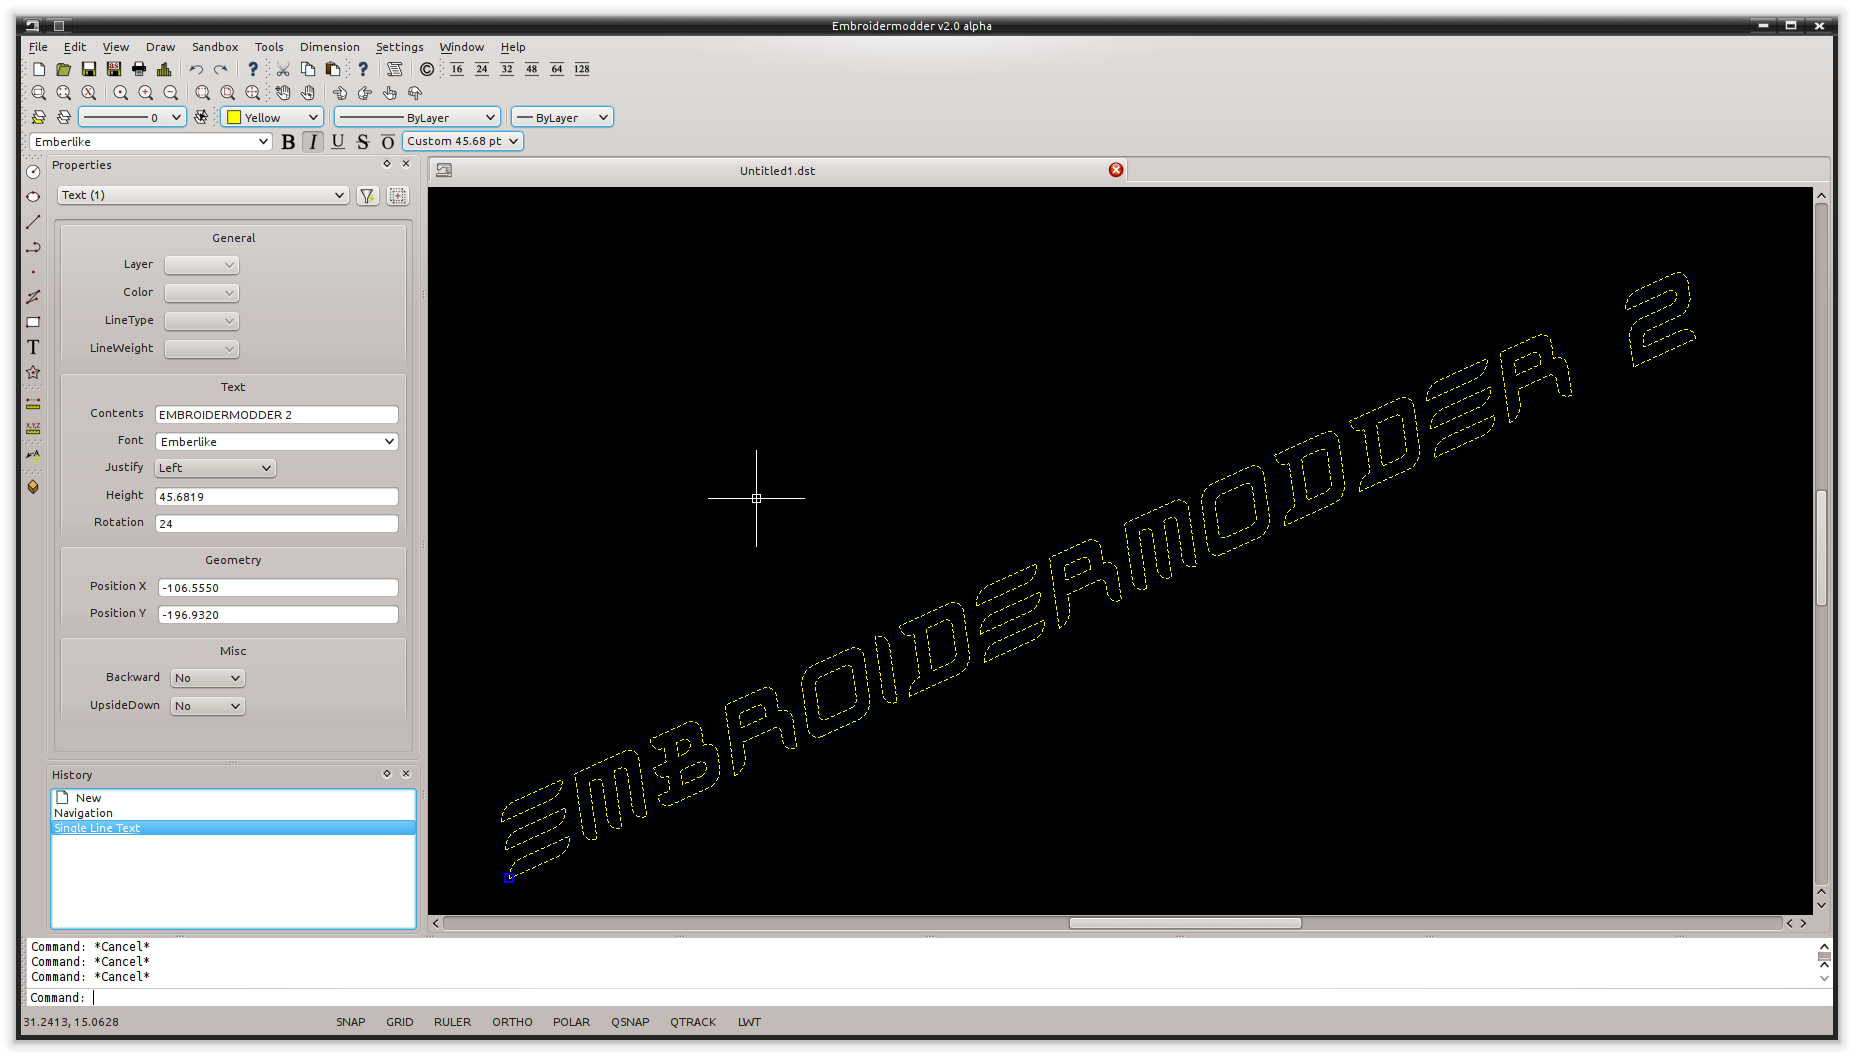
\includegraphics[width=0.9\textwidth]{images/features-text-1.png}

\subsection{Supports many formats}

Embroidery machines all accept different formats. There are so many formats available that it can sometimes be confusing whether a design will work with your machine.

Embroidermodder 2 supports a wide variety of embroidery formats as well as several vector formats, such as SVG and DXF. This allows you to worry less about which designs you can use.

\subsection{Batch Conversion}

Need to send a client several different formats? Just use libembroidery-convert, our command line utility which supports batch file conversion.

There are a multitude of formats to choose from:

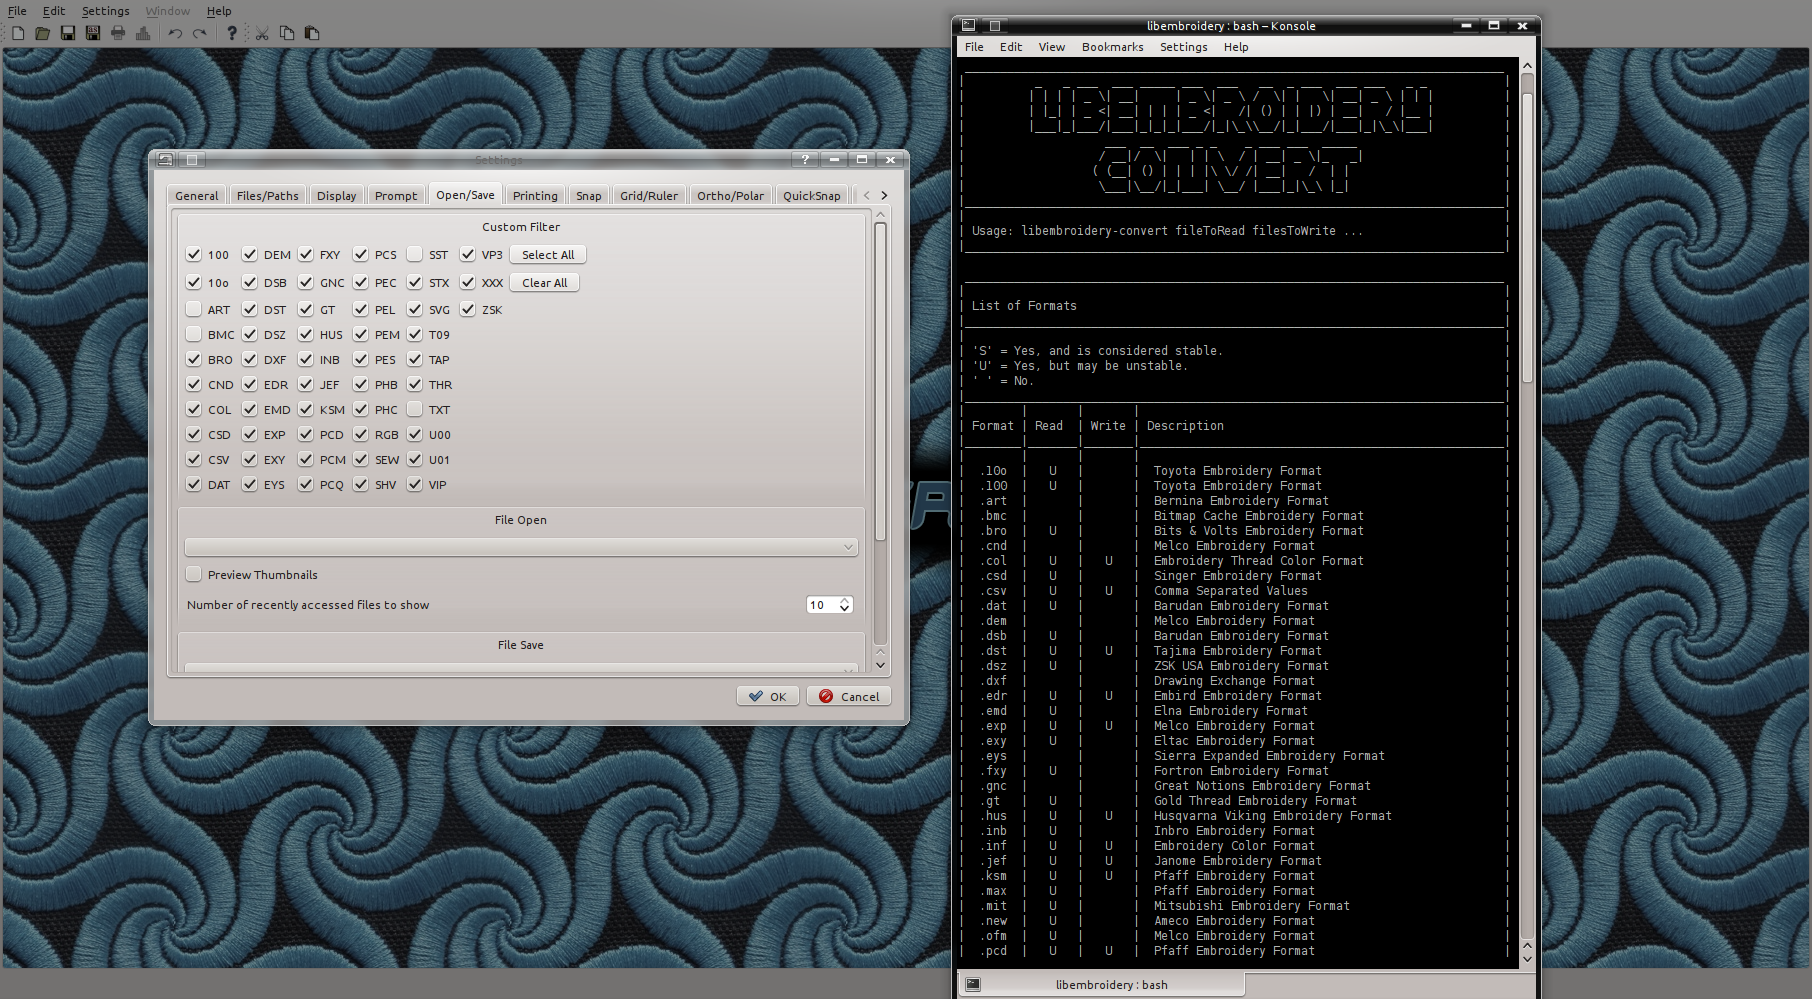
\includegraphics[width=0.9\textwidth]{images/features-formats-1.png}

\subsection{Scripting API}

If you've got programming skills and there is a feature that isn't currently available that you absolutely cannot live without, you have the capability to create your own custom commands for Embroidermodder 2. We provide an QtScript API which exposes various application functionality so that it is possible to extend the application without requiring a new release. If you have created a command that you think is worth including in the next release, just <a href=``contact.html``>contact us</a> and we will review it for functionality, bugs, and finally inclusion.

An Embroidermodder 2 command excerpt:

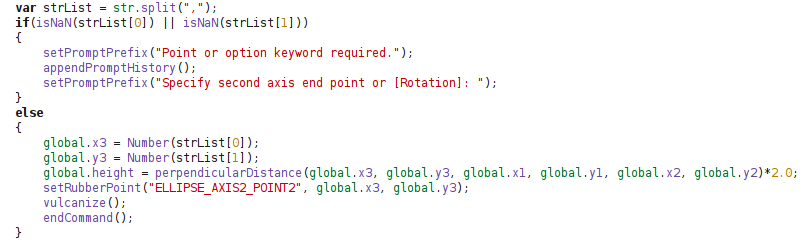
\includegraphics[width=0.9\textwidth]{images/features-scripting-1.png}

\section{Build and Install}

Assuming you already have the SDL2 libraries you can proceed to using the fast build, which assumes you want to build and test locally.

The fast build should be:

\begin{lstlisting}
    bash build.sh
\end{lstlisting}

or, on Windows:

\begin{lstlisting}
    .\build.bat
\end{lstlisting}

Then run using the `run.bat` or `run.sh` scripts in the build/ directory.

Otherwise, follow the instructions below.

If you plan to install the dev version to your system (we recommend you wait for the official installers and beta release first) then use the CMake build instead.

\subsection{Install on Desktop}

We recommend that if you want to install the development version you use the CMake build. Like this:

\begin{lstlisting}
    git submodule init
    git submodule update

    mkdir build
    cd build
    cmake ..
    cmake --build .
    sudo cmake --install .
\end{lstlisting}

These lines are written into the file:

\begin{lstlisting}
    ./build_install.sh
\end{lstlisting}

On Windows use the next section.

\section{.}

\emph{(UNDER MAJOR RESTRUCTURING, PLEASE WAIT FOR VERSION 2)}

Embroidermodder is a free machine embroidery application.
The newest version, Embroidermodder 2 can:

\begin{itemize}
\item edit and create embroidery designs
\item estimate the amount of thread and machine time needed to stitch a design
\item convert embroidery files to a variety of formats
\item upscale or downscale designs
\item run on Windows, Mac and Linux
\end{itemize}

For more information, see our website \cite{thewebsite}.

Embroidermodder 2 is very much a work in progress since we're doing a ground up rewrite to an interface in Python using the GUI toolkit Tk. The reasoning for this is detailed in the issues tab.

For a more in-depth look at what we are developing read the developer notes (link to dev notes section). This discusses recent changes in a less formal way than a changelog (since this software is in development) and covers what we are about to try.

Documentation

The documentation is in the form of the website (included in the `docs/`
directory) and the printed docs in this file.

\subsection{Development}

If you wish to develop with us you can chat via the contact email
on the [website]\url{https://www.libembroidery.org} or in the issues tab on the
[github page]\url{https://github.com/Embroidermodder/Embroidermodder/issues}.
People have been polite and friendly in these conversations and I (Robin)
have really enjoyed them.
If we do have any arguments please note we have a
[Code of Conduct](CODE\_OF\_CONDUCT.md) so there is a consistent policy to
enforce when dealing with these arguments.

The first thing you should try is building from source using the [build advice](link to build)
above. Then read some of the [development notes](link to dev notes.md) to get the general
layout of the source code and what we are currently planning.

\subsection{Testing}

To find unfixed errors run the tests by launching from the command line with:

\begin{lstlisting}
$ embroidermodder --test
\end{lstlisting}

then dig through the output. It's currently not worth reporting the errors, since
there are so many but if you can fix anything reported here you can submit a PR.

\section{Code Optimisations and Simplifications}

\subsection{Geometry}

The geometry is stored, processed and altered via libembroidery. See the Python specific part of the documentation for libembroidery for this. What the code in Embroidermodder does is make the GUI widgets to change and view this information graphically.

For example if we create a circle with radius 10mm and center at (20mm, 30mm) then fill it with stitches the commands would be

\begin{lstlisting}
from libembroidery import Pattern, Circle, Vector, satin
circle = Circle(Vector(20, 30), 10)
pattern = Pattern()
pattern.add_circle(circle, fill=satin)
pattern.to_stitches()
\end{lstlisting}

but the user would do this through a series of GUI actions:

\begin{enumerate}
\item Create new file
\item Click add circle
\item Use the Settings dialog to alter the radius and center
\item Use the fill tool on circle
\item Select satin from the drop down menu
\end{enumerate}

So EM2 does the job of bridging that gap.

\subsection{Postscript Support}

In order to safely support user contributed/shared data that can define, for example, double to double functions we need a consistent processor for these descriptions.

Embroidermodder backends to the postscript interpreter included
in libembroidery to accomplish this.

For example the string:

\begin{verbatim}
5 2 t mul add
\end{verbatim}

is equivalent to the expression:

\begin{verbatim}
2*t + 5
\end{verbatim}

The benefit of not allowing this to simply be a Python expression is that it is safe against malicious use, or accidental misuse. The program can identify whether the output is of the appropriate form and give finitely many calculations before declaring the function to have run too long (stopping equations that hang).

To see examples of this see the `assets/shapes/*.ps` files.

\subsection{SVG Icons}

To make the images easier to alter and restyle we could switch to svg icons. There's some code in the git history to help with this.

\subsection{The Actions System}

In order to simplify the development of a GUI that is flexible and easy to understand to new developers we have a custom action system that all user actions will go via an `actuator` that takes a string argument. By using a string argument the undo history is just an array of strings.

The C `action\_hash\_data` struct will contain: the icon used, the labels for the menus and tooltips and the function pointer for that action. There will be an accompanying argument for this function call, currently being drafted as `action\_call`. So when the user makes a function call it should contain information like the mouse position, whether special key is pressed etc.

\subsection{Accessibility}

Software can be more or less friendly to people with dylexia, partial sightedness, reduced mobility and those who don't speak English. Embroidermodder 2 has, in its design, the following features to help:

\begin{itemize}
\item icons for everything to reduce the amount of reading required
\item the system font is configurable: if you have a dyslexia-friendly font you can load it
\item the interface rescales to help with partial-sightedness
\item the system language is configurable, unfortunately the docs will only be in English but we can try to supply lots of images of the interface to make it easier to understand as a second language
\item buttons are remappable: XBox controllers are known for being good for people with reduced mobility so remapping the buttons to whatever setup you have should help
\end{itemize}

Note that most of these features will be released with version 2.1, which is planned for around early 2023.

\subsection{Sample Files}

Various sample embroidery design files can be found in the embroidermodder2/samples folder.

\subsection{Shortcuts}

A shortcut can be made up of zero or more modifier keys and at least one non-modifier key pressed at once.

To make this list quickly assessable, we can produce a list of hashes which are simply the flags ORed together.

The shortcuts are stored in the csv file ``shortcuts.csv'' as a 5-column table with the first 4 columns describing the key combination. This is loaded into the shortcuts `TABLE`. Each tick the program checks the input state for this combination by first translating the key names into indices for the key state, then checking for whether all of them are set to true.

\subsection{Removed Elements}

So I've had a few pieces of web infrastructure fail me recently and
I think it's worth noting. An issue that affects us is an issue that
can effect people who use our software.

\subsection{Qt and dependencies}

Downloading and installing Qt has been a pain for some users
(46Gb on possibly slow connections).

I'm switching to FreeGLUT 3 (which is a whole other conversation) which means we
can ship it with the source code package meaning only a basic build
environment is necessary to build it.

\subsection{Social Platform}

Github is giving me a server offline (500) error and is still giving a bad ping.

So... all the issues and project boards etc. being on Github is all well and good assuming that we have our own copies. But we don't if Github goes down or some other major player takes over the space and we have to move (again, since this started on SourceForge).

This file is a backup for that which is why I'm repeating myself between them.

\subsection{Pandoc Documentation}

The documentation is, well better in that it's housed in the main repository,
but I'm not a fan of the ``write once build many'' approach as it means
trying to weigh up how 3 versions are going to render.

Can we treat the website being a duplicate of the docs a non-starter?
I'd be happier with tex/pdf only and (I know this is counter-intuitive) one
per project.

\subsection{OpenGL}

OpenGL rendering within the application. This will allow for
Realistic Visualization - Bump Mapping/OpenGL/Gradients?

This should backend to a C renderer or something.

\subsection{Configuration Data Ideas}

Embroidermodder should boot from the command line
regardless of whether it is or is not installed (this helps with testing and
running on machines without root). Therefore, it can create an initiation file
but it won't rely on its existence to boot: `~/.embroidermodder/config.json`.

\begin{itemize}
\item Switch colors to be stored as 6 digit hexcodes with a \texttt{\#}.
\item We've got close to a hand implemented ini read/write setup in `settings.py`.
\end{itemize}

\subsection{Distribution}

When we release the new pip wheel we should also package:

* `.tar.gz` and `.zip` source archive.
* Debian package
* RPM package

Only do this once per minor version number.

\subsection{Scripting Overhaul}

Originally Embroidermodder had a terminal widget, this is why we removed it.

\begin{quote}
\textbf{ROBIN}

I think supporting scripting within Embroidermodder doesn't make sense.

All features that use scripting can be part of libembroidery instead.
Users who are capable of using scripting won't need it, they can alter their embroidery files in CSV format, or import pyembroidery to get access.
It makes maintaining the code a lot more complicated, especially if we move away from Qt.
Users who don't want the scripting feature will likely be confused by it, since we say that's what libembroidery, embroider and pyembroidery are for.

How about a simpler ``call user shell`` feature? Similar to texmaker we just call system on a batch or shell script supplied by the user and it processes the file directly then the software reloads the file. Then we aren't parsing it directly.

I don't want to change this without Josh's support because it's a fairly major change.

\textbf{JOSH}

I totally agree.

I like the idea of scripting just so people that know how to code could write their own designs without needing to fully build the app. Scripting would be a very advanced feature that most users would be confused by. Libembroidery would be a good fit for advanced features.

Now we are using Python (again, sort of) this would be a lot more natural,
perhaps we could boot the software without blocking the shell so they can
interact? TODO: Screenshot a working draft to demonstrate.
\end{quote}

\subsection{Perennial Jobs}

\begin{enumerate}
\item Check for memory leaks
\item Clear compiler warnings on `-Wall -ansi -pedantic` for C.
\item Write new tests for new code.
\item Get Embroidermodder onto the current version of libembroidery.
\item PEP7 compliance.
\item Better documentation with more photos/screencaps.
\end{enumerate}

\subsection{Full Test Suite}

(This needs a hook from Embroidermodder to embroider's full test suite.)

The flag `--full-test-suite` runs all the tests that have been written.
Since this results in a lot of output the details are both to stdout
and to a text file called `test\_matrix.txt`.

Patches that strictly improve the results in the `test\_matrix.txt` over
the current version will likely be accepted and it'll be a good place
to go digging for contributions. (Note: strictly improve means that
the testing result for each test is as good a result, if not better.
Sacrificing one critera for another would require some design work
before we would consider it.)

\subsection{Symbols}

Symbols use the SVG path syntax.

In theory, we could combine the icons and symbols systems, since they could be rendered once and stored as icons in Qt. (Or as textures in FreeGLUT.)

Also we want to render the patterns themselves using SVG syntax, so it would save on repeated work overall.


\section{Features}

\subsection{Bindings}

Bindings for libembroidery are maintained for the languages we use internally in the project, for other languages we consider that the responsibility of other teams using the library.

So libembroidery is going to be supported on:

\begin{itemize}
\item C (by default)
\item C++ (also by default)
\item Java (for the Android application MobileViewer)
\item Swift (for the iOS application iMobileViewer)
\end{itemize}

For C\# we recommend directly calling the function directly
using the DllImport feature:

\begin{lstlisting}
[DllImport("libembroidery.so", EntryPoint="readCsv")]
\end{lstlisting}

see this StackOverflow discussion for help: \url{https://stackoverflow.com/questions/11425202/is-it-possible-to-call-a-c-function-from-c-net}.

For Python you can do the same using ctypes: \url{https://www.geeksforgeeks.org/how-to-call-a-c-function-in-python/}.

\subsection{Other Supported Thread Brands}

The thread lists that aren't preprogrammed into formats but are indexed in the data file for the purpose of conversion or fitting to images/graphics.

\begin{itemize}
\item Arc Polyester
\item Arc Rayon
\item Coats and Clark Rayon
\item Exquisite Polyester
\item Fufu Polyester
\item Fufu Rayon
\item Hemingworth Polyester
\item Isacord Polyester
\item Isafil Rayon
\item Marathon Polyester
\item Marathon Rayon
\item Madeira Polyester
\item Madeira Rayon
\item Metro Polyester
\item Pantone
\item Robison Anton Polyester
\item Robison Anton Rayon
\item Sigma Polyester
\item Sulky Rayon
\item ThreadArt Rayon
\item ThreadArt Polyester
\item ThreaDelight Polyester
\item Z102 Isacord Polyester
\end{itemize}
